\subsubsection{Aufgabe der Komponente}
Durch das Radar können Geräte, auf welchen ebenfalls die Anwendung Sharknet installiert ist, in räumlicher Nähe ausfindig gemacht und angezeigt werden. Es nutzt dabei die Verhaltensweise der WiFi-Komponente, bei der in regelmäßigen Abständen Geräteinformationen an alle Geräte in der Nähe geschickt werden. Diese Geräteinformationen werden vom Radar empfangen, gebündelt und dem Benutzer dann auf dem Gerät als Liste angezeigt. Der Benutzer kann anschließend anhand dieser Geräteliste einen Chat eröffnen. Neben der Eröffnung von Chats ist diese Geräteliste außerdem wichtig für die Broadcast-Komponente, da die Broadcast Nachricht an alle Geräte geschickt wird, die sich auf dieser Liste befinden.

\subsubsection{Architektur}

\subsubsubsection{Überlick}\label{ch:radaroverview}
Im folgenden UML-Klassendiagramm sind alle Bestandteile der Radar-Komponente von SharkNet abgebildet.
\begin{figure}[H]
	\centering
	\hspace*{1cm}
	\makebox[\linewidth][c]{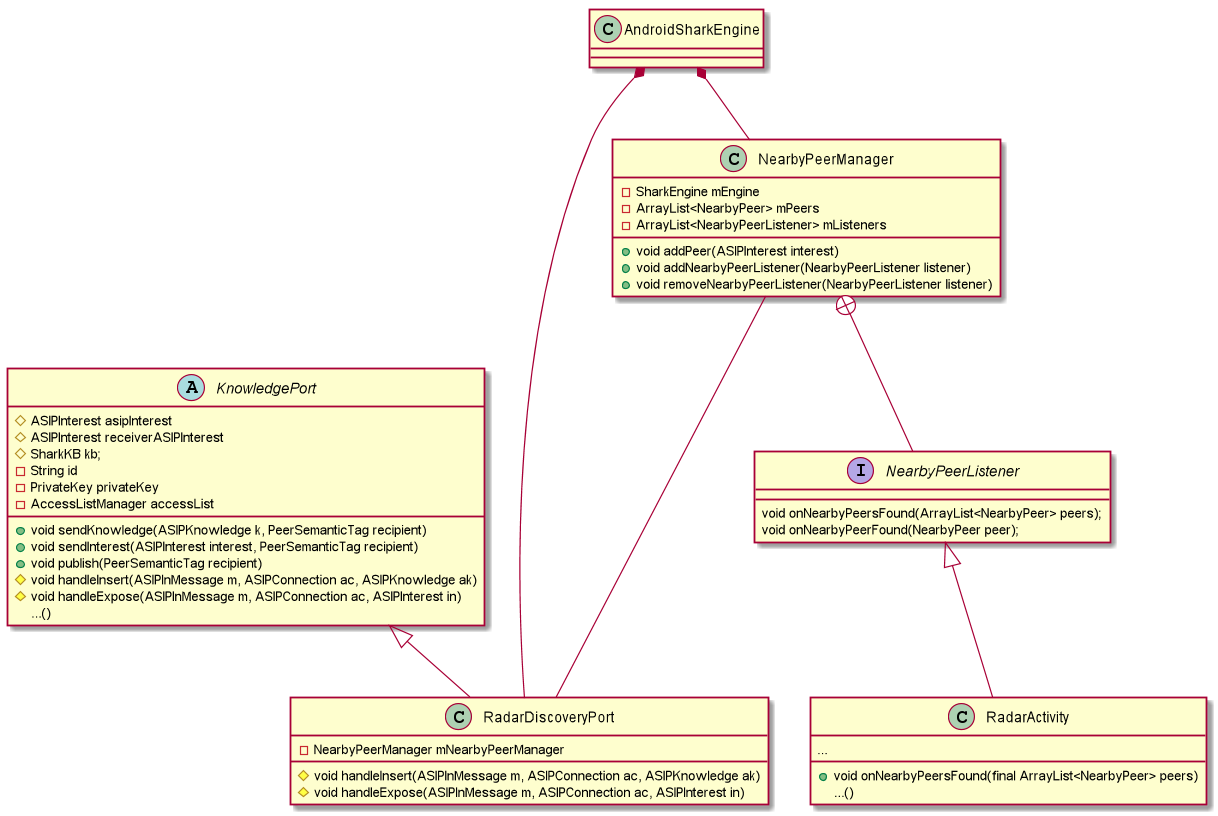
\includegraphics[width=1.1\linewidth]{radar/images/radar.png}}%
	\caption{Die Radar Klassen im Überblick}
	\label{fig:radarhAll}
\end{figure}
Die eingangs erwähnte Geräteliste befindet sich als Attribut innerhalb der Klasse \textit{NearbyPeerManager}. Die Klasse enthält das Interface \textit{NearbyPeerListener}, welches für die Benachrichtigungen im Falle von neu gefundenen Geräten zuständig ist. Android Activities wie die \textit{RadarActivity} oder aber auch die \textit{BroadcastActivity} implementieren dieses Interface, um über eine stets über alle Geräte in der Nähe informiert zu sein. Der \textit{RadarDiscoveryPort} ist die Schnittstelle zwischen Anwendung und Shark Framework. Die im Grundlagenkapitel Kapitel erwähnten Knowledge-Port-Methoden \textit{handleInsert()} und \textit{handleExpose()} werden benötigt, weil die Geräte ihre Informationen in Form von ASIP-Interessen versenden. Diese Interessen werden nach dem Empfang dann auf der Ebene des Frameworks durch die Methode \textit{handleInsert()} verarbeitet und anschließend auf der Ebene der Anwendung dem Benutzer dargestellt.

\subsubsubsection{Schnittstellendefinitionen}\label{ch:radarinterfaces}
lore

\subsubsection{Nutzung}
Die Komponente kann über die \textit{startDiscovery()} Methode der \textit{AndroidSharkEngine} gestartet werden.

\subsubsubsection{Code}
lore

\subsubsubsection{Deployment / Runtime}
lore


\subsubsection{Test}
lore


\subsubsection{Ausblick}
lore 
\newpage